%%%%%%%%%%%%%%%%%%%%%%%%%%%%%%%%%%%%%%%%%
% University Assignment Title Page 
% LaTeX Template
% Version 1.0 (27/12/12)
%
% This template has been downloaded from:
% http://www.LaTeXTemplates.com
%
% Original author:
% WikiBooks (http://en.wikibooks.org/wiki/LaTeX/Title_Creation)
%
% License:
% CC BY-NC-SA 3.0 (http://creativecommons.org/licenses/by-nc-sa/3.0/)
% 
% Instructions for using this template:
% This title page is capable of being compiled as is. This is not useful for 
% including it in another document. To do this, you have two options: 
%
% 1) Copy/paste everything between \begin{document} and \end{document} 
% starting at \begin{titlepage} and paste this into another LaTeX file where you 
% want your title page.
% OR
% 2) Remove everything outside the \begin{titlepage} and \end{titlepage} and 
% move this file to the same directory as the LaTeX file you wish to add it to. 
% Then add \input{./title_page_1.tex} to your LaTeX file where you want your
% title page.
%
%%%%%%%%%%%%%%%%%%%%%%%%%%%%%%%%%%%%%%%%%

%----------------------------------------------------------------------------------------
%	PACKAGES AND OTHER DOCUMENT CONFIGURATIONS
%----------------------------------------------------------------------------------------

\documentclass[12pt]{article}
\usepackage[catalan]{babel}
\usepackage[utf8]{inputenc}
\usepackage{float}
\usepackage{graphicx}
\usepackage{wrapfig}
\usepackage{lscape}
\usepackage{rotating}
\usepackage{epstopdf}
\usepackage{makeidx}

\makeindex
\begin{document}

\begin{titlepage}

\newcommand{\HRule}{\rule{\linewidth}{0.5mm}} % Defines a new command for the horizontal lines, change thickness here

\center % Center everything on the page
 
%----------------------------------------------------------------------------------------
%	HEADING SECTIONS
%----------------------------------------------------------------------------------------

\textsc{\LARGE Universitat de Barcelona}\\[1.5cm] % Name of your university/college
\textsc{\Large Client-Servidor}\\[0.5cm] % Major heading such as course name
\textsc{\large Enfonsar la flota}\\[0.5cm] % Minor heading such as course title

%----------------------------------------------------------------------------------------
%	TITLE SECTION
%----------------------------------------------------------------------------------------

\HRule \\[0.4cm]
{ \huge \bfseries Pràctica 1}\\[0.4cm] % Title of your document
\HRule \\[1.5cm]
 
%----------------------------------------------------------------------------------------
%	AUTHOR SECTION
%----------------------------------------------------------------------------------------



% If you don't want a supervisor, uncomment the two lines below and remove the section above
\Large \emph{Author:}\\
Christian José \textsc{Soler}\\
Nicolás Martín \textsc{Forteza Ocaña}\\[3cm] % Your name

%----------------------------------------------------------------------------------------
%	DATE SECTION
%----------------------------------------------------------------------------------------

{\large \today}\\[3cm] % Date, change the \today to a set date if you want to be precise

%----------------------------------------------------------------------------------------
%	LOGO SECTION
%----------------------------------------------------------------------------------------

%\includegraphics{Logo}\\[1cm] % Include a department/university logo - this will require the graphicx package
 
%----------------------------------------------------------------------------------------

\vfill % Fill the rest of the page with whitespace

\end{titlepage}
\addcontentsline{toc}{section}{Índice alfabético}
\printindex
\section*{Introducció}
En esta práctica se nos pide implementar el juego célebre \textit{Hundir la flota} para que juegan diferents clientes contra un mismo servidor.

El objetivo del juego es adivinar la situación de los barcos del enemigo y hundirlos indicando las coordenadas donde creemos que están. Para que cliente y servidor se entiendan entre ellos se debe implementar el protocolo espeficado en el enunciado.

Nuestra finalidad pues será implementar este programa, aprendiendo así a utilizar los mecanismos de programación cliente-servidor de Java, como la API de Sockets y de Selectors.

El cliente deberá tener un modo manul, un modo con IA sencilla y un modo con IA más compleja para jugar contra el servidor. El servidor debe tener los mismos modos, exceptuando el manual.

Tendremos que implementar dos versiones de servidor que para cliente serán ambos transparentes: Un servidor donde cada cliente será gestionado por un thread aparte y otro, donde el servidor recibirá los mensajes de los clientes mediante un selector y gestionará todas las partidas a medida que van llegando los mensajes de los clientes.

\newpage
\section*{Proceso de desarrollo}
Inicialmente, tuvimos que plantear bien el proyecto y hacer un buen diagrama de clases, ya que eso nos permitió que nuestro código sea robusto  y a la larga, nos ahorró mucho tiempo y previno posibles errores.

Nuestro primer objetivo fue pues crear una versión local del juego, donde el cliente juega contra su propio tablero, pudiendo así probar la mecánica del juego básico, sin comunicación.

Una vez arreglados los errores de flujo básico, comenzamos a preparar la comunicación y simultáneamente empezamos a poner la base del servidor con Threads. En este punto nos dimos cuenta que estos proyectos compartían tanto código que merecía la pena crear una librería común, llamada swd-core,  donde vinieran todas aquellas clases que ambos usan. Eso se debe a que nos parecía poco óptimo tener que modificar el mismo código varias veces.

Como hemos ido aplicando bastantes patrones de diseño y creamos swd-core, hemos podido reducir considerablemente el tiempo que necesitamos para hacer funcionar la comunicación entre cliente-servidor.

Cuando conseguimos tener estable la versión cliente-servidor con threads, pasamos a la última tarea de esta entrega: crear el servidor con selectores. Nos inspiramos en el ejemplo que se nos dio en clase.

Completadas todas las tareas, hicimos nuestras últimas pruebas en local, y posteriormente, en la sesión de test. Con eso acabamos el trabajo.

\newpage
\section*{Detalles del desarrollo}


\newpage
\section*{Annex}
\begin{sidewaysfigure}[ht]
    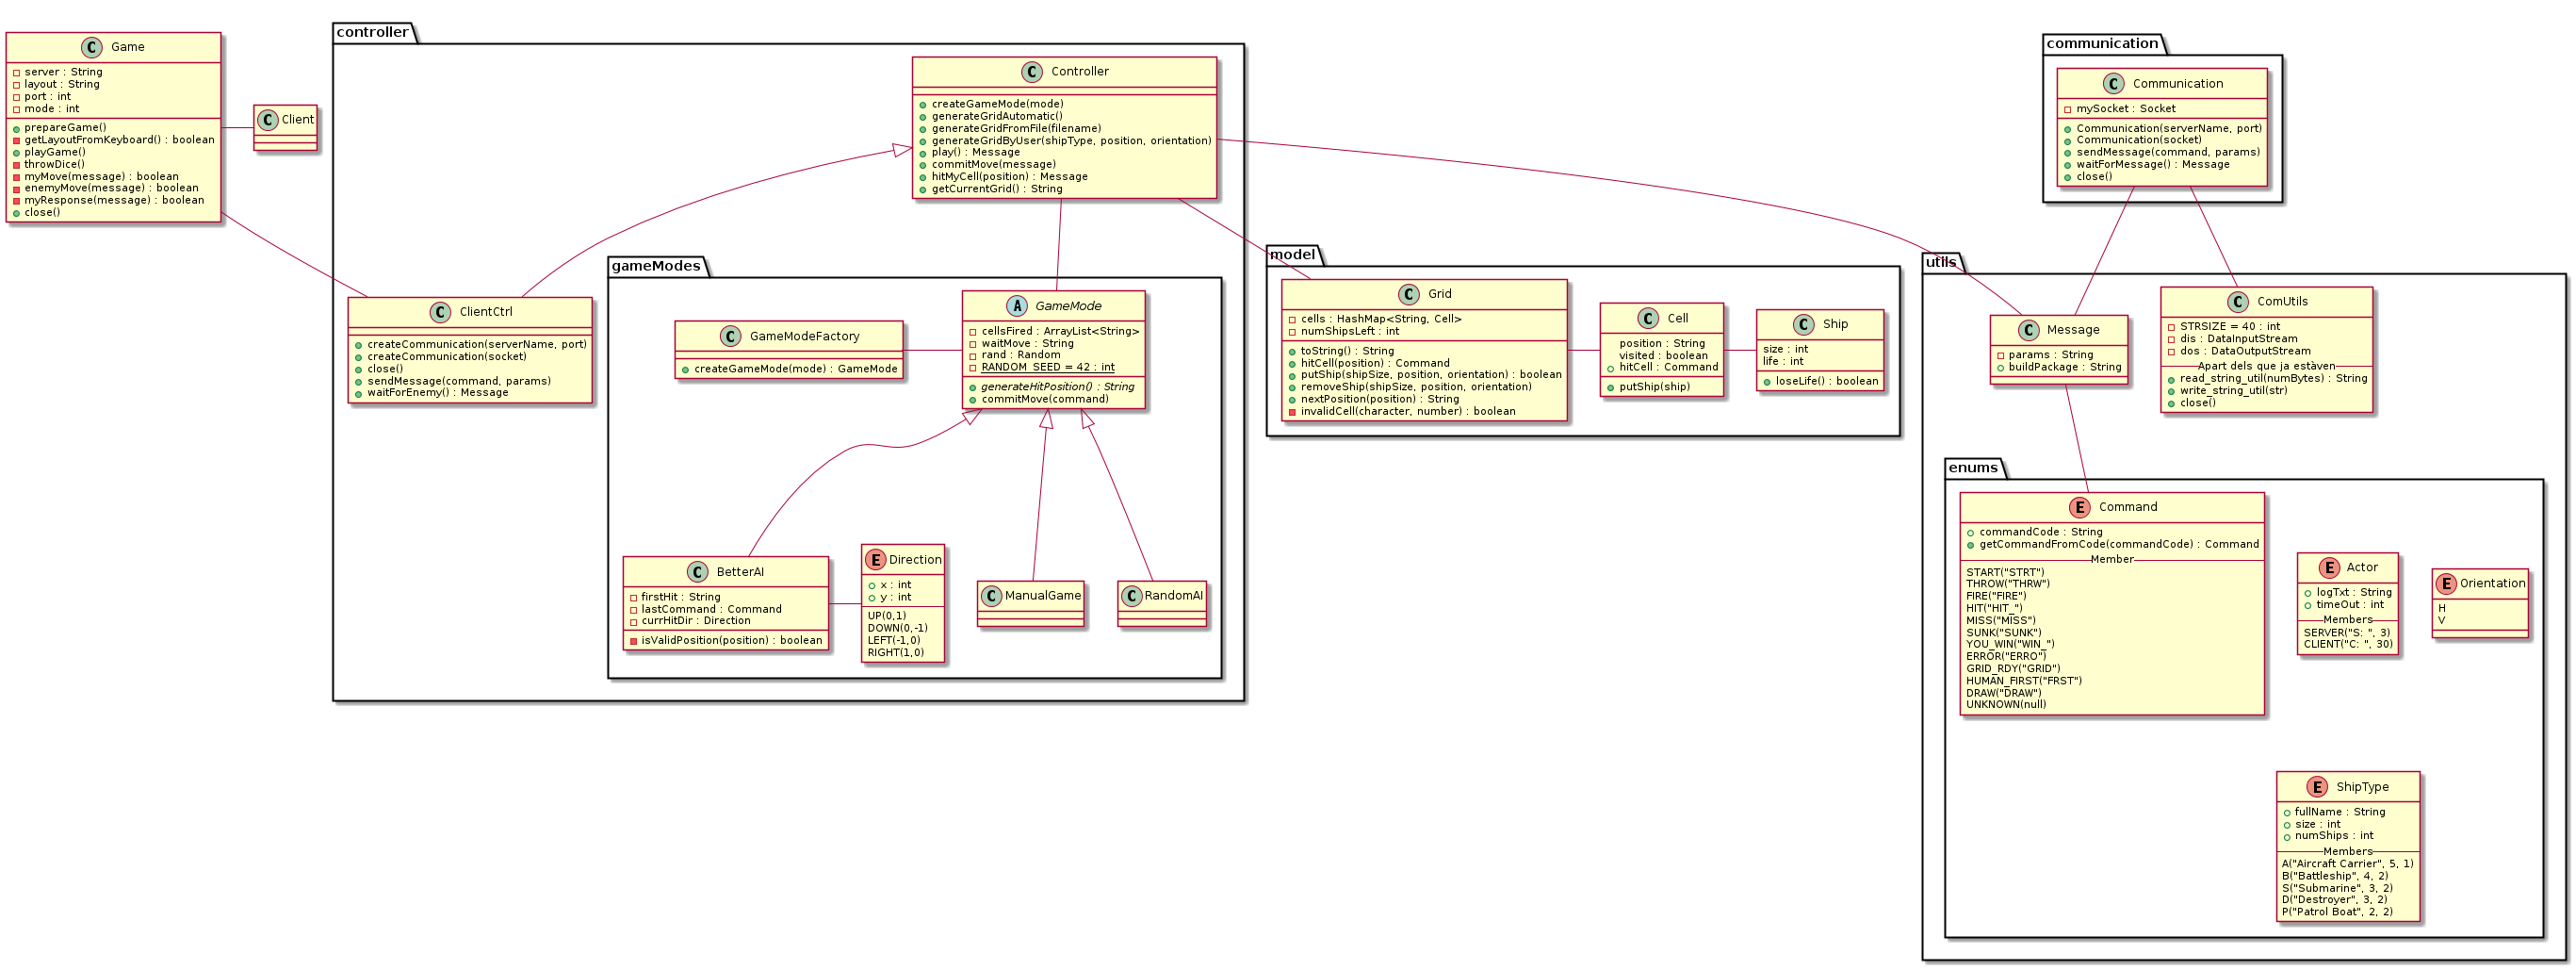
\includegraphics[width=\textwidth,height=\textheight,keepaspectratio]{../diagrams/class-diagrams/clientClasses.png}
    \caption{Client Diagram}
    \label{fig:PropProf}
\end{sidewaysfigure}
\begin{sidewaysfigure}[ht]
    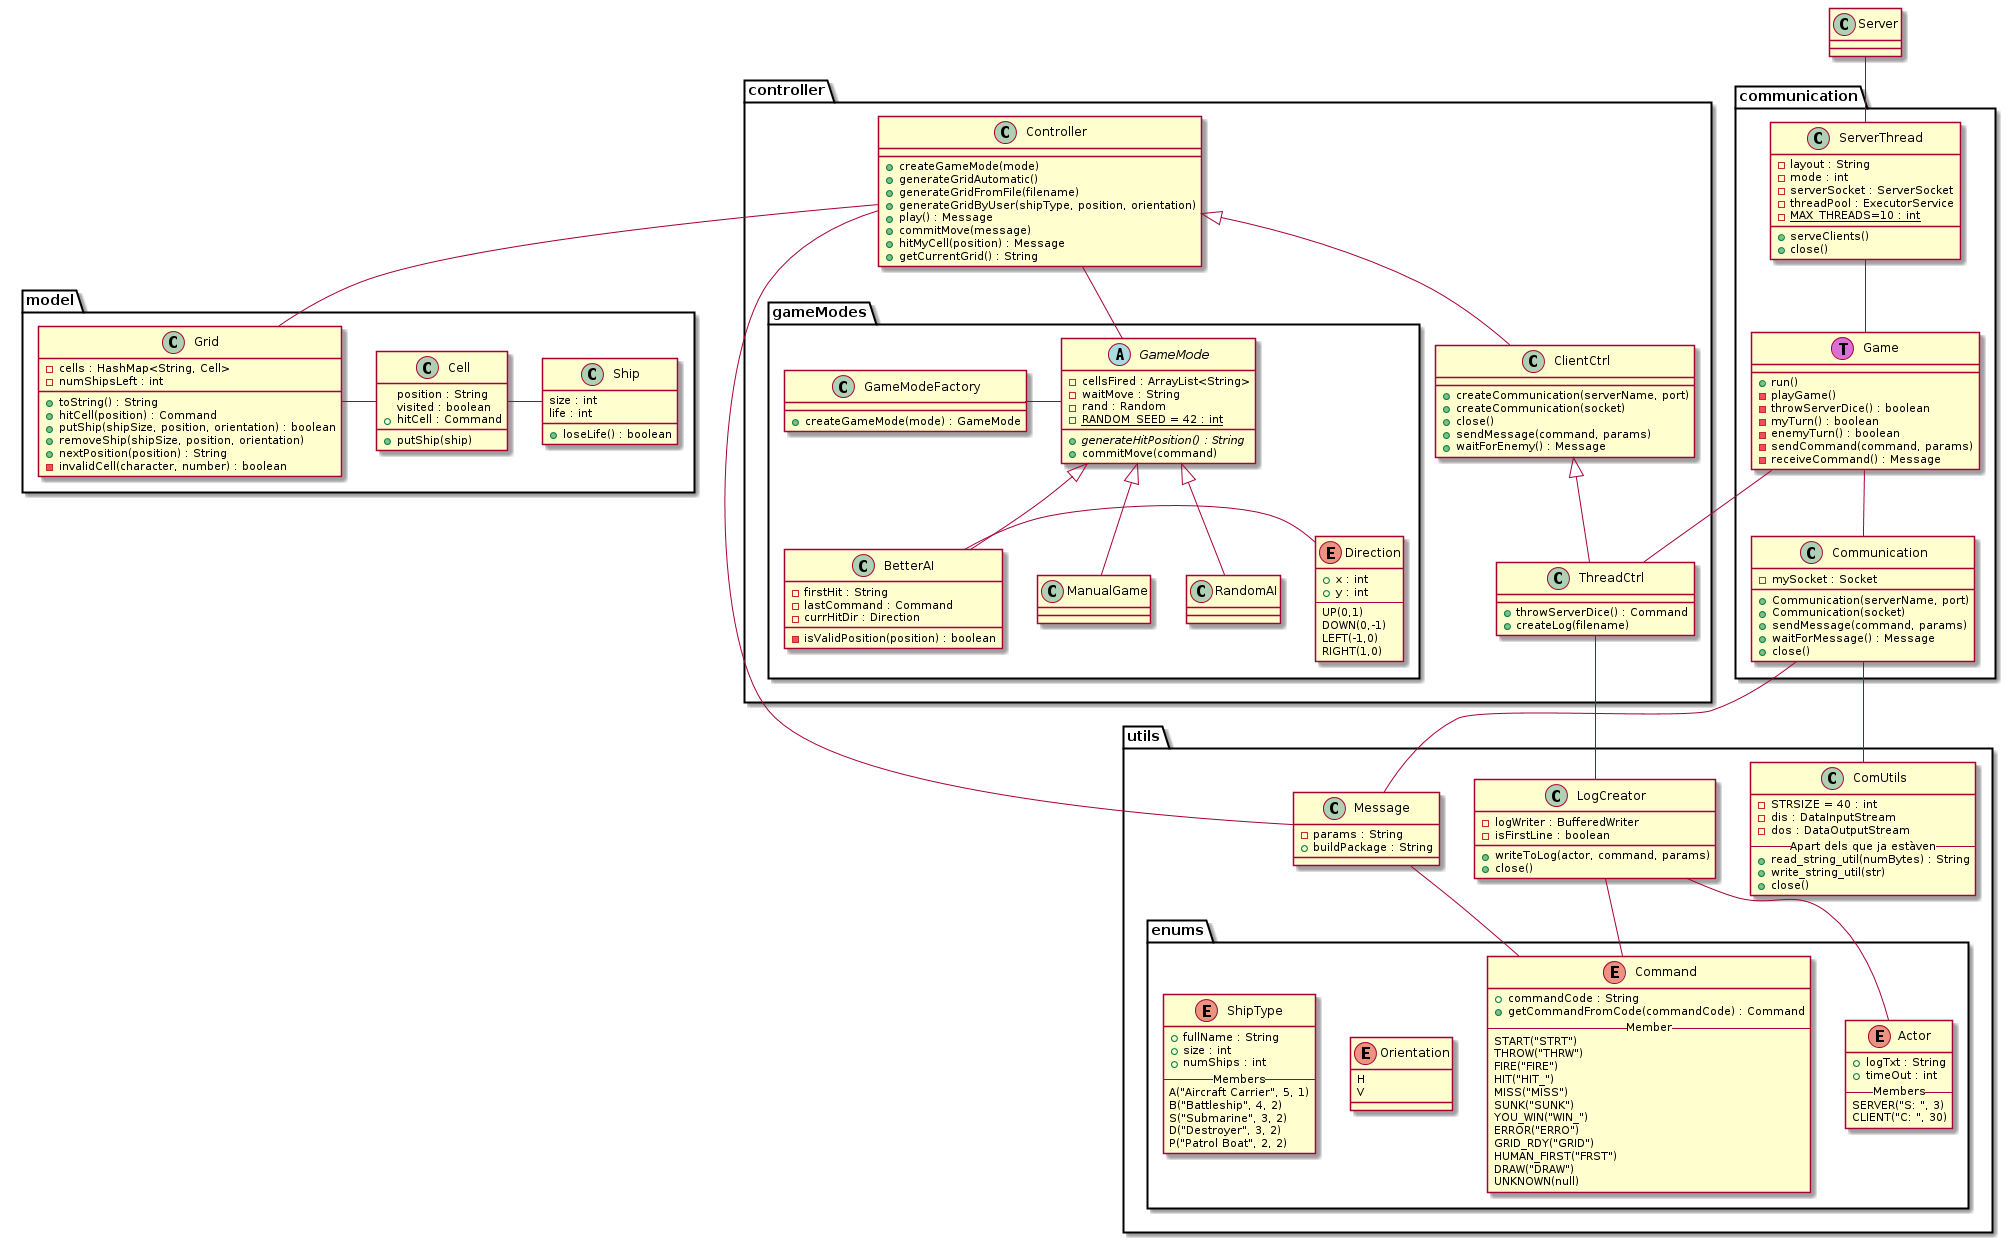
\includegraphics[width=\textwidth,height=\textheight,keepaspectratio]{../diagrams/class-diagrams/threadsClasses.png}
    \caption{Threads-Server Diagram}
    \label{fig:PropProf}
\end{sidewaysfigure}
\begin{sidewaysfigure}[ht]
    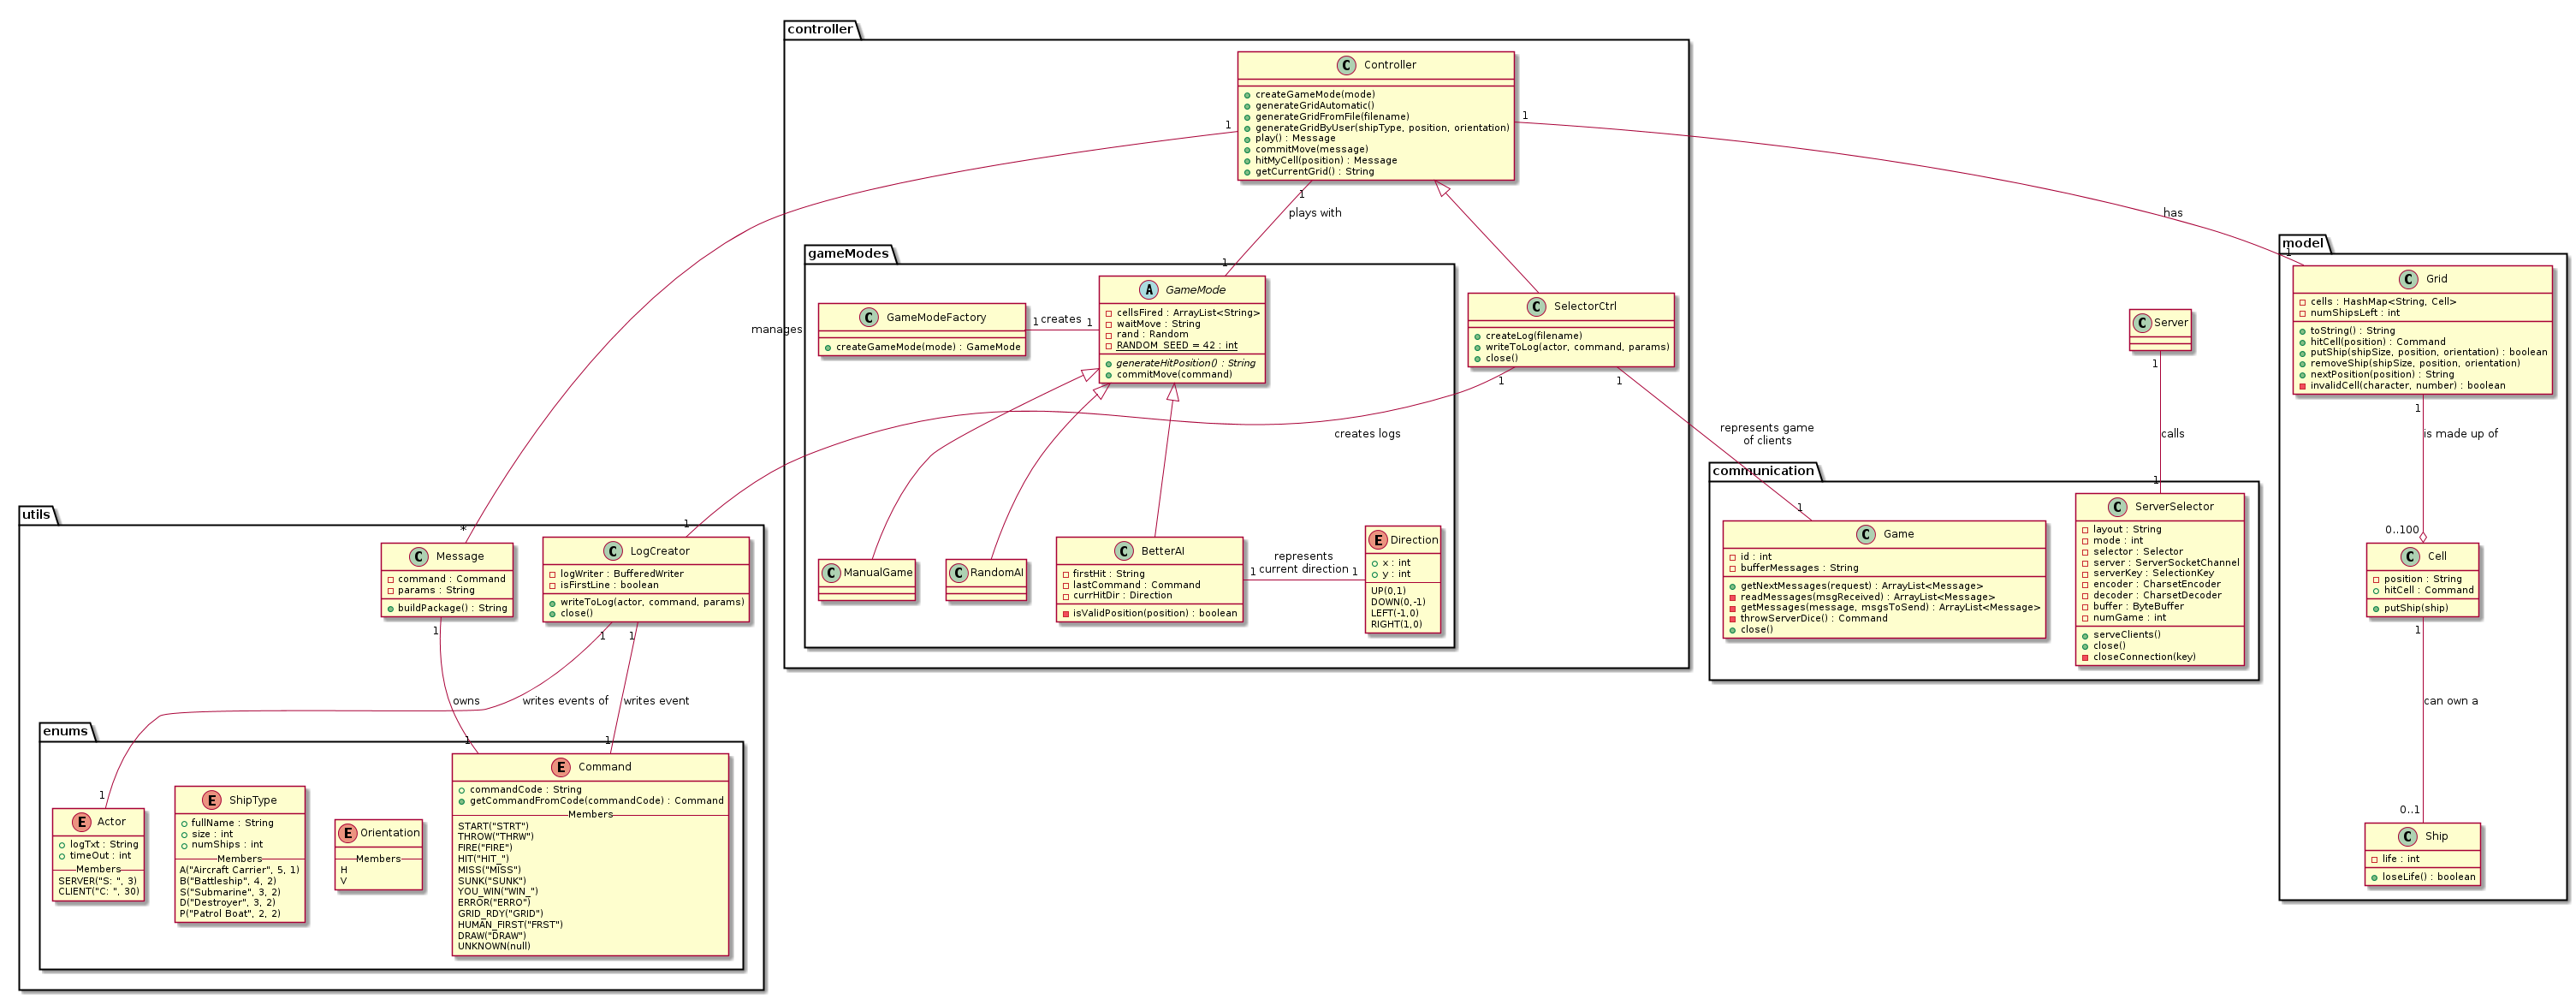
\includegraphics[width=\textwidth,height=\textheight,keepaspectratio]{../diagrams/class-diagrams/selectorClasses.png}
    \caption{Selector-Server Diagram}
    \label{fig:PropProf}
\end{sidewaysfigure}

\end{document}	